% !TEX encoding = UTF-8 Unicode
%!TEX root = thesis.tex
% !TEX spellcheck = en-US
%%=========================================

\chapter{Profiling Data}
\label{appendix-b}

\begin{figure}[ht!]
\centering
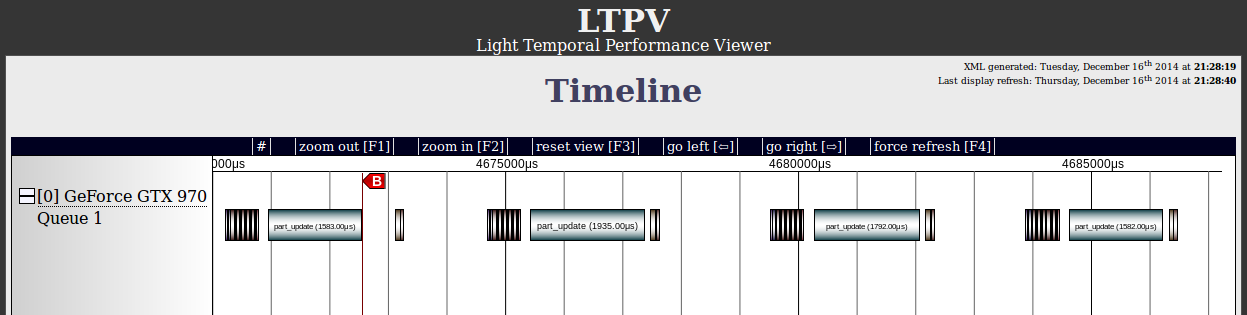
\includegraphics[width=\textwidth]{fig/profiling/1m_32}
\caption{Profiling data for 1 million particles, 32x32x32 windfield}
\label{fig:1m_32}
\end{figure}

\begin{figure}[ht!]
\centering
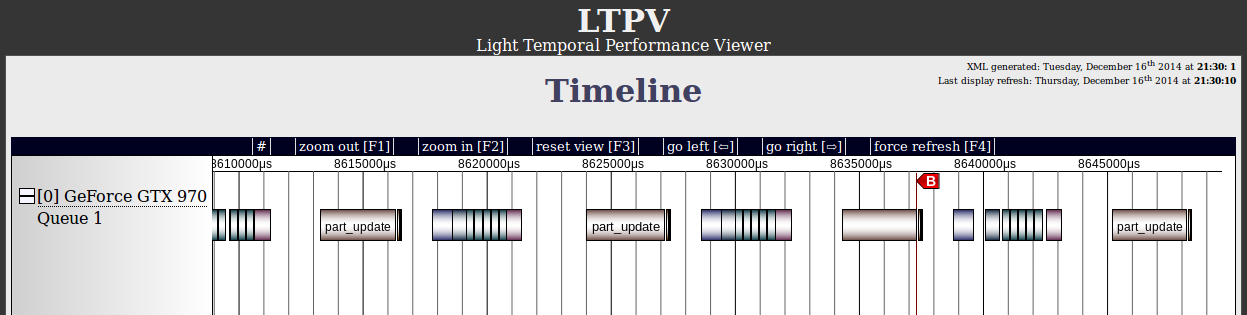
\includegraphics[width=\textwidth]{fig/profiling/1m_128}
\caption{Profiling data for 1 million particles, 32x32x32 windfield}
\label{fig:1m_128}
\end{figure}

\begin{figure}[ht!]
\centering
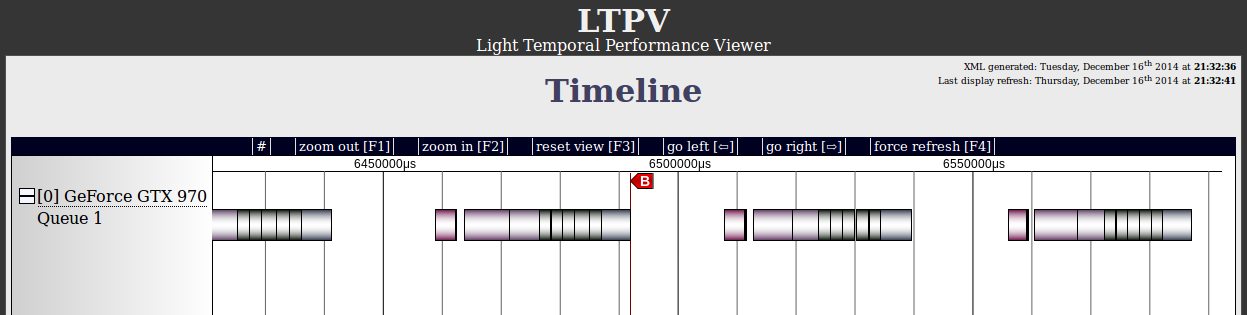
\includegraphics[width=\textwidth]{fig/profiling/1m_256}
\caption{Profiling data for 1 million particles, 32x32x32 windfield}
\label{fig:1m_256}
\end{figure}

\begin{figure}[ht!]
\centering
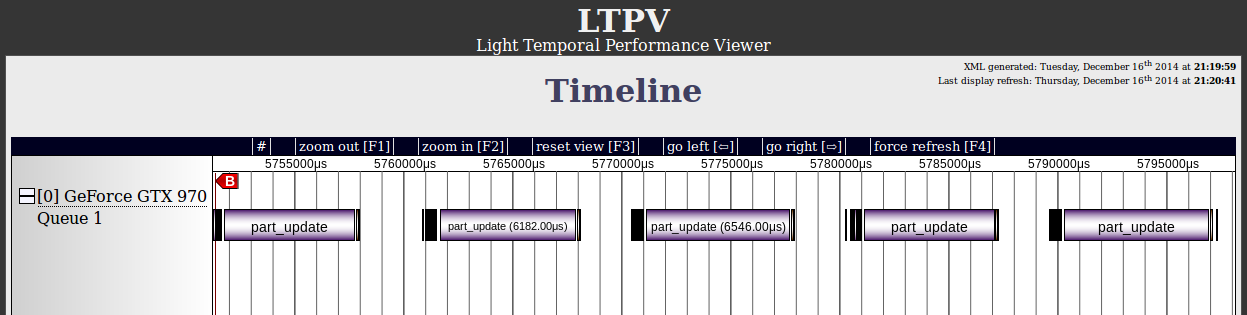
\includegraphics[width=\textwidth]{fig/profiling/4m_32}
\caption{Profiling data for 4 million particles, 32x32x32 windfield}
\label{fig:4m_32}
\end{figure}

\begin{figure}[ht!]
\centering
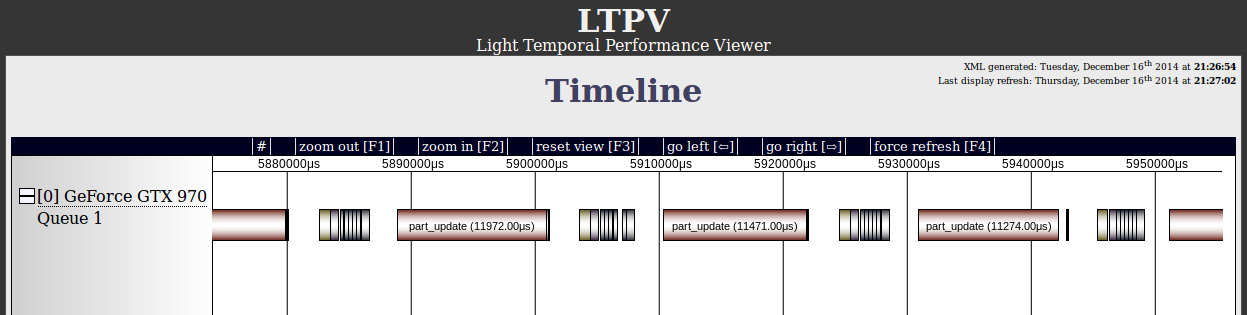
\includegraphics[width=\textwidth]{fig/profiling/4m_128}
\caption{Profiling data for 4 million particles, 128x128x128 windfield}
\label{fig:4m_128}
\end{figure}

\begin{figure}[ht!]
\centering
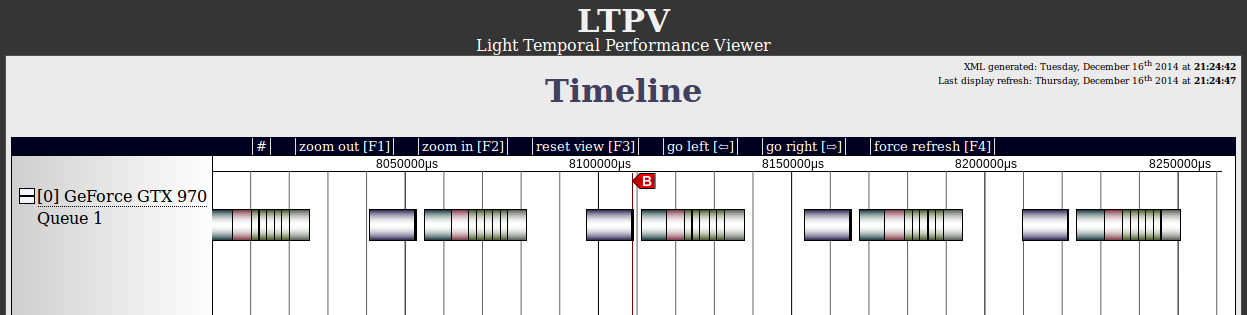
\includegraphics[width=\textwidth]{fig/profiling/4m_256}
\caption{Profiling data for 4 million particles, 256x256x256 windfield}
\label{fig:4m_256}
\end{figure}

\begin{figure}[ht!]
\centering
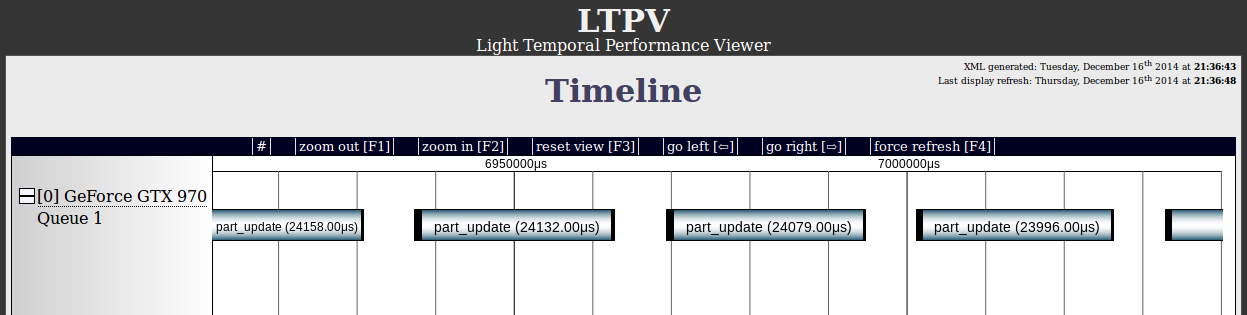
\includegraphics[width=\textwidth]{fig/profiling/16m_32}
\caption{Profiling data for 16 million particles, 32x32x32 windfield}
\label{fig:16m_32}
\end{figure}

\begin{figure}[ht!]
\centering
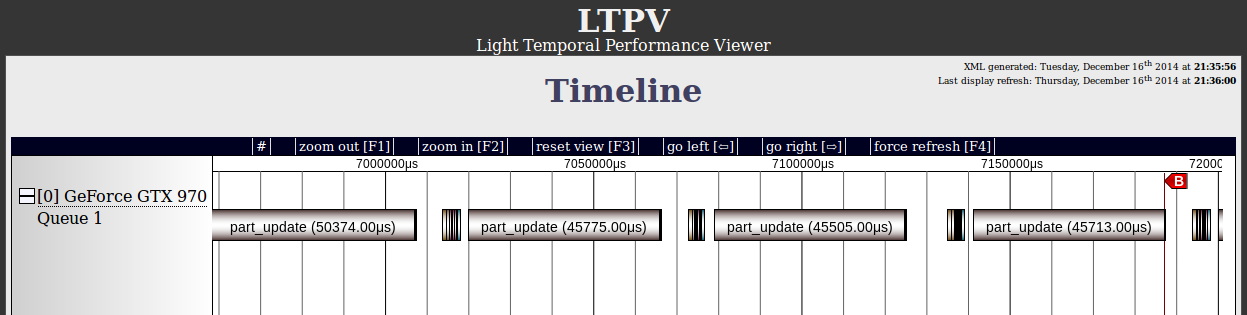
\includegraphics[width=\textwidth]{fig/profiling/16m_128}
\caption{Profiling data for 16 million particles, 128x128x128 windfield}
\label{fig:16m_128}
\end{figure}

\begin{figure}[ht!]
\centering
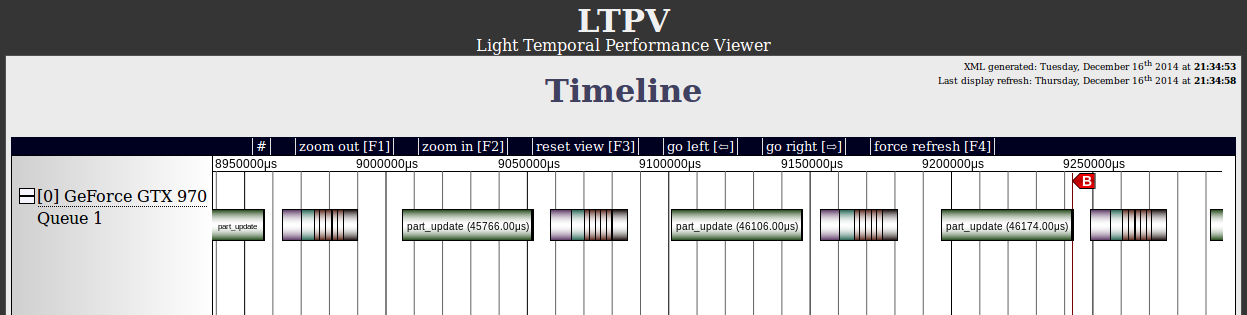
\includegraphics[width=\textwidth]{fig/profiling/16m_256}
\caption{Profiling data for 16 million particles, 256x256x256 windfield}
\label{fig:16m_256}
\end{figure}